\documentclass[12pt,letterpaper]{article}
\usepackage[top=2cm,left=2cm,right=2cm,bottom=2cm]{geometry}
\usepackage[utf8]{inputenc}
\usepackage[T1]{fontenc}  
\usepackage{ae}
\usepackage{amsmath,amssymb}
\usepackage{setspace}
\usepackage{graphicx}
\usepackage{indentfirst}
\usepackage{url}
\usepackage{color}
\usepackage{cite}
\usepackage{gensymb}
\usepackage{subcaption}
\usepackage{hyperref}
\usepackage{epigraph}
\usepackage{mathtools}
\usepackage{mathrsfs}
\usepackage{epstopdf}

\definecolor{red}{rgb}{1.0,0.0,0.0}
\definecolor{green}{rgb}{0.01,0.75,0.24}
\definecolor{blue}{rgb}{0.0,0.0,1.0}

\newcommand{\ket}[1]{| #1 \rangle}
\newcommand{\bra}[1]{\langle #1 |}
\newcommand{\expected}[1]{ \langle #1 \rangle}
\newcommand{\product}[2]{\langle #1 | #2 \rangle}
\newcommand{\pib}{\boldsymbol{\pi}}
\newcommand{\sigmab}{\boldsymbol{\sigma}}
\newcommand{\project}{\large Research Project Renewal  \vskip 0.1cm}
\newcommand{\asu}{Physics Department \\ Arizona State University}

\begin{document}
\onehalfspacing
%\doublespace
\title{\project {\Large \textbf{Quantum Monte Carlo Calculations of Nucleon 
Systems and Cold Atom Gases}} \vspace{0cm}}
\author{
{\bf PIs: Kevin E. Schmidt}, Arizona State University \\
{\bf Stefano Gandolfi}, Los Alamos National Laboratory
}
\date{\today}
\maketitle

\section*{Abstract}

This research project renewal request is for 1,000,000 SUs on SuperMIC.
We describe our progress on cold atom gases simulations, and nucleon systems 
calculations.
One of the proposed goals is to include explicitly the pionic degrees of 
freedom in 
the nuclear Monte Carlo simulations.
We also have been developing improved trial wave functions for nuclei and 
nuclear matter, and we intend to continue our research by extending these wave 
functions to other nucleon systems.
In summary, we will continue to employ
Quantum Monte Carlo methods to study nucleon systems and cold atom gases, by 
using  
our large-scale highly-parallel code, which 
has been successfully used to calculate properties of cold gases, nuclear 
matter, 
neutron matter, and medium-mass nuclei in the past.

\section{Research Objectives}

This allocation renewal request is intended to provide the computational 
resources 
to continue to carry out the project \textit{Quantum Monte Carlo (QMC) 
Calculations of 
Nucleon Systems} supported by the National Science Foundation grant 
PHY-1404405, and related projects.

Many nuclear processes in our universe occur under extreme conditions in 
supernovae and neutron stars. The properties of nuclei and nuclear matter 
under these conditions, which are difficult or impossible to reproduce in 
the laboratory, must necessarily be calculated theoretically. These data are 
needed to understand astrophysically important systems and processes such as 
neutron rich matter, neutron stars, supernovae, and r-process 
nucleosynthesis and neutrino scattering. The quantum many-particle methods 
developed within this project have broad applications across many areas of 
physics, including nuclear physics, cold atomic gas research, and electronic 
structure. Methods 
previously developed within this project have been applied in each of these 
areas.

The results of this project are relevant for the nuclear physics program at 
the Department of Energy Office of Science, that has identified the 
knowledge of the structure of nuclei and nuclear matter as one of the most 
important scientific questions in nuclear physics in the most recent Nuclear 
Science Advisory Committee long-range plan.

The detailed development of the initial proposal is discussed 
in the document ``\textit{Progress Report}", which was submitted alongside this 
one. In this document we summarize the advances we have achieved, in addition 
to the proposed plan for the current cycle.

In Sec.~\ref{sec:cold} we describe our progress on cold fermionic gases, 
including the study of a vortex line excitation in the unitary Fermi gas, and 
core structure vortex properties of two-dimensional Fermi gases.
The inclusion of explicit pion field contributions in simulations of nucleon 
systems is discussed in Sec.~\ref{sec:pions}.
In Sec.~\ref{sec:improved} we present our study of improved wave functions for 
nuclei and nuclear matter.

\subsection{Strongly paired fermionic systems of cold atoms}
\label{sec:cold}

Strongly paired fermions are important in many contexts, for example: nuclei, 
atoms, condensed matter systems, and even neutron stars. 
Cold atom gases provide a unprecedented clean way to the deal with the 
fermionic many-body problem. The ingenious usage of magnetic fields can be used 
to tune the interatomic interactions of the systems, thus reaching a wide 
spectrum of interaction strengths.
Cold atom experiments can provide direct tests of the
equation of state and the pairing gap in the strongly
paired regime, and provide a benchmark
of many-body theories in these systems.

Until very recently, superfluids were classified as either bosonic or 
fermionic. The Bose-Einstein condensate (BEC) theory was developed to describe 
bosonic fluids. On the other hand, the Bardeen-Cooper-Schrieffer (BCS) theory 
was first conceived to describe pairing instability, arising from weak 
interactions, in a highly degenerate Fermi gas. 
Later it was realized that the BEC and BCS schemes are limit cases of a 
continuum of interactions. The possibility of tuning parameters in order to 
observe the change from one paradigm to the other was conceptually interesting, 
but real enthusiasm came from the experimental realization of the
three-dimensional (3D) BEC-BCS crossover \cite{reg04}. Right in the middle of 
this 
crossover lies a strongly interacting
state, the unitary Fermi gas, with remarkable properties.

In our Startup allocation we studied
vortices in the unitary Fermi gas \cite{mad16}. We reported diffusion Monte 
Carlo results for the ground-state of unpolarized spin-1/2 fermions in a 
cylindrical container and properties of the system with a vortex-line 
excitation. We calculated quantities such as: density profiles, the ground-
state energy per particle, the superfluid pairing gap, and the excitation 
energy per particle.

We used the current allocation to study the core structure of two-dimensional 
Fermi gas vortices in the BEC-BCS crossover region.
The study of cold Fermi gases has proven to be a very rich research 
field, and the investigation of low-dimensional systems has become an 
active area in this context \cite{gio08,blo08}. Particularly,
the two-dimensional (2D) Fermi gas has attracted much interest 
recently. It was 
the object of several theoretical investigations 
\cite{ran89,ran90,pet03,mar05,tem07,zha08}, but its experimental 
realization, using a highly anisotropic potential, was a milestone in 
the study of these systems \cite{kir10}. Many other studies have been 
carried out since \cite{ore11,mak14}. QMC methods 
were successfully employed to compute several properties of the BEC-BCS 
crossover.
The fact that a fully attractive potential in 
2D always support a bound-state, and the ability to vary the 
interaction strength over the entire BEC-BCS crossover regime offers 
rich 
possibilities for the study of these systems.
	
The presence of quantized vortices is an indication of a superfluid 
state in both Bose and Fermi systems. In 3D, much progress has been 
made \cite{bul03,sen06,mad16}, including the observation of vortex 
lattices in a strongly interacting rotating Fermi gas of $^6$Li 
\cite{zwi05}. With the recent progress on the 2D Fermi gases, it seemed 
natural to also extend the theoretical study of vortices to these 
systems. Interest 
is further augmented in 2D, where a Berezinksii-Kosterlitz-Thouless 
transition \cite{ber70,kos72} could take place at finite temperatures, 
and pairs of vortices and antivortices would eventually condense to form 
a 
square lattice \cite{bot06}.

We studied properties of a single vortex in a 2D Fermi gas. We 
considered the ground-state to be a disk with hard walls and total 
angular momentum zero, and the vortex excitation corresponds to each 
fermion pair having angular momentum $\hbar$. 

Our findings were summarized in the article
``Core structure of two-dimensional Fermi gas vortices
in the BEC-BCS crossover region" \cite{mad17}, which has been submitted to the 
Physical 
Review A journal.
We reported $T=0$ diffusion Monte Carlo results for 
the ground-state and vortex excitation of unpolarized spin-1/2 fermions 
in a two-dimensional disk. We investigated how vortex core structure 
properties behave over the BEC-BCS crossover. We calculated the vortex 
excitation energy, density profiles, and vortex core properties related 
to the current. We found a density suppression at the vortex core on 
the BCS side of the crossover, and a depleted core on the BEC limit. 
Size-effect dependencies in the disk geometry were carefully studied.

\subsection{QMC simulations with explicit contributions from the pion field}
\label{sec:pions}

Most QMC simulations of nuclear matter model particles interacting via
instantaneous two- and three-body
potentials \cite{car15}. Usually these potentials are either
phenomenological or are derived from chiral 
effective field theories for nuclear structure by approximately integrating 
out the field
degrees of freedom. Our goal is to include explicitly the low energy degrees 
of freedom of the pion field in the QMC
simulations, while the high energy degrees of freedom will be included in 
the instantaneous potentials. We will develop an expression for the low 
energy components of the pion field, the potential for the high energy 
degrees of freedom, the Hamiltonian of the system and suitable wave functions 
for this problem.

We have been developing wave functions for systems with $A\leqslant 4$ 
nucleons, and we are in the process of implementing them in the code. Once that 
has been achieved, simulations with one nucleon can help us to determine its 
bare mass. Simulations with two nucleons will serve as benchmarks to our choice 
of two-body potentials. The comparison of our results for light-nuclei 
properties with other numerical calculations and experiments will shed light on 
the explicit contributions of the pion field.  

\subsection{Improved trial wave functions for nuclei and nuclear matter}
\label{sec:improved}

In QMC calculations, the results are dependent on the accuracy of the trial 
wave
function employed to guide the random walk. We have recently introduced
a linearly pair-correlated wave function which has greatly improved the
convergence of our results\cite{gan14}. We are now working on
including multiple pair correlations to study their effect. 
We have written codes to efficiently handle the large number of
matrix operations required to include these additional correlations.

In the past year we have been able to add quadratic correlations to the trial 
wave function that we use in nuclear Monte Carlo calculations. These additional 
correlations have caused the energies to decrease for the nuclei $^4$He and 
$^{16}$O, as well as for symmetric nuclear matter. We plan to publish these 
results shortly.
These linear and quadratic correlations come from an expansion of the 
exponential correlation. We plan to include the full set of exponential 
correlations in the nuclear trial wave function. We then plan to use these 
improved wave function to investigate the clustering of nucleons into alpha 
particles in mostly neutron matter.
We intend to study the convergence of variational and auxiliary field
diffusion Monte Carlo with these new wave functions for nuclei and
nuclear matter with $A \stackrel{<}{~} 40$.

\section{Computational Methods}
\label{sec:comp_met}

We use QMC methods, in particular Auxiliary Field Diffusion Monte Carlo 
(AFDMC) methods, which have proven to be very successful in calculating 
ground-state properties including momentum distributions, as we have shown 
in our article for Reviews of Modern Physics \cite{car15}. The AFDMC code 
has been successfully used to calculate properties of nuclear matter, 
neutron matter, and medium-mass nuclei \cite{gan14}. The results of 
Ref.~\cite{gan12} showed the relation between the symmetry energy and 
properties 
of neutron stars.

We have written a large-scale highly-parallel code to achieve high precision 
calculations for many properties of medium-mass nuclei. The AFDMC code 
calculates the
ground-state of the nucleus through a branching random walk algorithm, and it
can be used to compute other properties including radii and momentum 
distributions.

\subsection{Algorithm and implementation}

The AFDMC code has been developed by the investigators of this project. The 
AFDMC method is used to extract the ground-state component of the system 
from the variational ansatz describing the system. This is done with a 
projection in imaginary-time, i.e. we calculate
\begin{equation}
\label{eq:dif}
\lim_{n\rightarrow\infty}\left[ e^{-H\delta\tau}\right]^n \Psi_T(R,S) 
\rightarrow \Psi_0(R',S'),
\end{equation}
where $R =(r_1, \cdots, r_N)$ are the coordinates of nucleons, $S = (s_1, 
\cdots, s_N)$ are complex numbers indicating their spin and isospin 
projections, and $\Psi_T(R,S)$ is a trial variational wave function. The 
algorithm is a branching random walk that requires the diagonalization of 
$3N \times 3N$ matrices ($N$ is the number of particles) at each step of the 
random walk. AFDMC is written in Fortran90 and MPI, and it uses the vendor 
optimized BLAS and LAPACK libraries to perform matrix diagonalizations at 
each step.

The AFDMC algorithm is a variant of Diffusion Monte Carlo, where each step 
involves:
\begin{enumerate}
\item Diffuse nucleon’s positions, $R \rightarrow R'$ according to the 
kinetic energy $T$ of the Hamiltonian.
\item Rotate nucleon’s spins, $S \rightarrow S'$, according to the spin and 
isospin-dependent potential.
\item Calculate the weight $W$ of the new configuration, and generate $n$ 
replicas of the new configuration according to $n = [W + \eta]$, where 
$\eta$  is a random number uniformly distributed from 0 to 1.
\end{enumerate}

This algorithm is implemented by considering
a collection of configurations (called \textit{walkers})
that are simultaneously evolved in imaginary-time. The parallelization is 
accomplished
by spreading the configurations among the nodes. However, AFDMC is not 
embarrassingly parallel because the branching term generates fluctuations in 
the number of configurations, of the order up to 10\%, and the calculation 
of observables requires an average over walkers at the same imaginary-time. 
We employ a dynamic load rebalancing after
each time step to redistribute walkers across nodes.

\section{Application efficiencies}

The AFDMC code is written in Fortran90 and MPI. We describe in detail the 
performance and scaling of our code in the additional document submitted 
with this proposal. The most relevant feature that we present in that 
document is the scaling in XSEDE resources, namely Stampede and SuperMIC.

We used our startup allocation (TG-PHY140003, PI Kevin Schmidt) to test the 
performance of the code on Stampede. Up to 4096 cores, the 
largest number tested, the code scales strongly, Fig.~\ref{fig:stampede}.
During the current allocation (TG-PHY160027), we verified that our code also 
scales strongly on SuperMIC, Fig.~\ref{fig:supermic}, up to 2560 cores (the 
largest number tested), although we intend to perform 
simulations with a maximum number of 1000 cores.

\begin{figure}[!htb]
\centering
\begin{subfigure}{.45\textwidth}
  \centering
  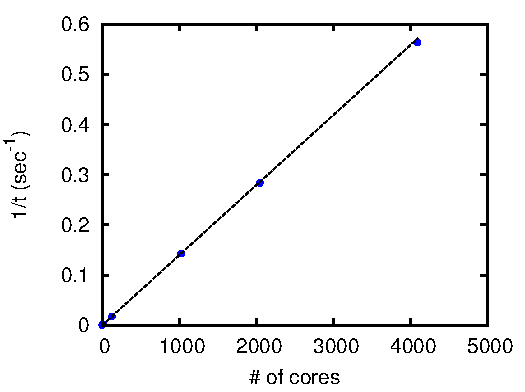
\includegraphics[width=\textwidth]{stampede.pdf}
  \caption{}
  \label{fig:stampede}
\end{subfigure}%
\hspace{0.01\textwidth}
\begin{subfigure}{.45\textwidth}
  \centering
  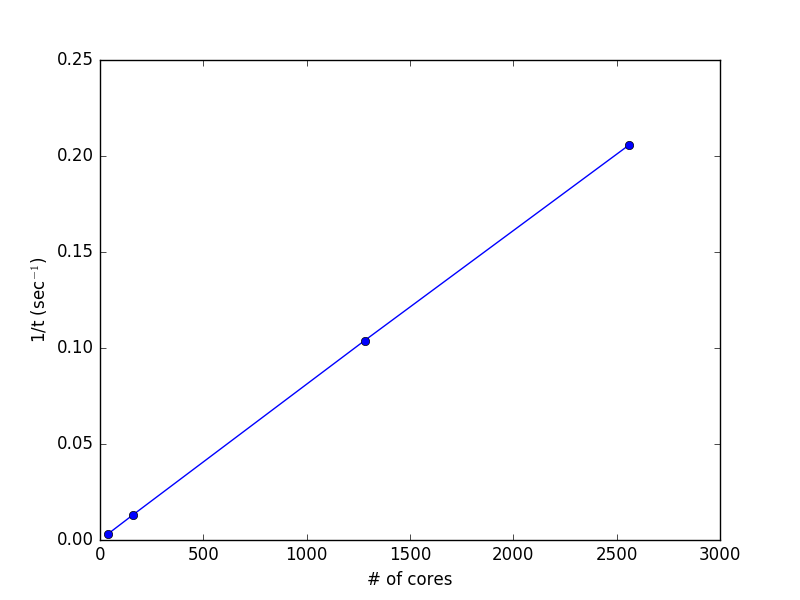
\includegraphics[width=\textwidth]{supermic.png}
  \caption{}
  \label{fig:supermic}
\end{subfigure}
\caption{Scaling on Stampede (a) and SuperMIC (b) using the time to propagate 
10000 configurations of an $^{16}$O nucleus for 100 steps.}
\label{fig:scaling}
\end{figure}

\section{Computational Research Plan and Justification for Requested 
Resources}

As discussed in Sec. \ref{sec:comp_met}, the simulations depend on a trial 
variational wave function. The variational parameters are determined using 
the stochastic reconfiguration method \cite{cas04}. Once these parameters 
are determined, we can proceed with the computation of physical quantities 
of interest. We base our estimates on the amount of SUs and storage used in 
\cite{car15} 
and references therein.

\subsection{QMC simulations with explicit contributions from the pion field}

We want to perform simulations with different system 
sizes, ranging from one nucleon plus the pion field up to four nucleons plus 
the pion field, a total of four systems. Several runs are needed for each 
system, because we have to investigate the behavior of properties as a function 
of the box size and number of pion modes, for example.

For each system we require:
\begin{itemize}
	\item variational optimization of the parameters: for these systems the 
	average amount of SUs necessary for the optimization is approximately 
	40,000 SUs.
	\item production runs: longer runs are necessary to compute quantities 
	such as energy of the system, density and other distribution functions, 
	with small variances. We estimate 80,000 SUs for these computations.
\end{itemize}

\subsection{Improved QMC simulations for nuclei and nuclear matter}

We want to do energy calculations on three systems, $^4$He, $^{16}$O, and 
symmetric nuclear matter using the new exponential correlations to compare the 
trial wave function with the linear and quadratic correlations. To do this we 
will need to optimize a new set of parameters. We estimate that this will 
require 20,000 SUs for development, 40,000 SUs to optimize the variational 
parameters for the new correlations, and 180,000 SUs to calculate the energies 
for the three nuclear systems mentioned above.

With this improved wave function we will be investigating the clustering of 
alpha particles in mostly neutron matter. We will be doing calculations for a 
variety of densities to investigate the clustering dependence on density. We 
estimate that this will require 20,000 SUs for development, 40,000 SUs to 
optimize the code for mostly neutron matter, and 180,000 SUs to calculate the 
clustering at a variety of densities.

\subsection{Summary of the requested resources}

We present in Table \ref{tab:SUs} the amount of SUs requested for each task.
We are requesting a total of 1,000,000 SUs on SuperMIC.
We also included SUs for the code 
development, in order to ensure performance and scaling during execution.

\begin{table}[htbp]
\centering
\caption{Justification for the requested amount of SUs}
\begin{tabular}{|l|r|r|r|}
\hline
 & \multicolumn{1}{c|}{\textbf{Explicit pion field}} & \multicolumn{ 2}{c|}
 {\textbf{Improved QMC simulations}} \\ \hline
 & \multicolumn{1}{l|}{} & \multicolumn{1}{l|}{Exp. correlations} & 
 \multicolumn{1}{l|}{Alpha particle clustering} \\ \hline
Development & 40,000 & 20,000 & 20,000 \\ \hline
Variational optimization & 160,000 & 40,000 & 40,000 \\ \hline
Production & 320,000 & 180,000 & 180,000 \\ \hline
Subtotal & 520,000 & 240,000 & 240,000 \\ \hline\hline
\multicolumn{ 4}{|c|}{\textbf{Total: 1,000,000 SUs}} \\ \hline
\end{tabular}
\label{tab:SUs}
\end{table}

As for storage needs, we request the default value of 5 GB per user. The size 
of input, 
output and configuration files is of approximately 50 MB per system. As the 
simulations are independent, there is no need to store all of them at the 
same time at SuperMIC. We are capable of handling the post-processing of the 
simulations in our local computing environment at Arizona State University.

\section{Additional considerations}

We believe that we have enough funding, through the NSF grant, and qualified 
staff to complete the work plan described in this project.

\subsection{Qualifications of the PIs and team}

\textbf{PIs}

\underline{Kevin Schmidt}
Kevin Schmidt in collaboration with Stefano Fantoni developed the
auxiliary field diffusion Monte Carlo method. With collaborators
he performed the first diffusion and auxiliary field quantum
Monte Carlo calculations for paired fermions.  He is a fellow of
the American Physical society and has published more than 140 papers.

\underline{Stefano Gandolfi} is a nationally and 
internationally recognized scientist in Many-Body Nuclear Theory. During the 
past 4 years he has published 29 papers and given 31 invited talks, 
including many at major national and international conferences. He has about 
2,500 citations on Google Scholar. As a result of his excellent work, 
Gandolfi received the International Union of Pure and Applied Physics prize 
for young researchers in nuclear physics in 2013. He has led a program in 
Quantum Monte Carlo at the Institute of Nuclear Theory in 2013, among other
conferences in 2017 and 2018.

\textbf{Graduate students}

\underline{Lucas Madeira} is a PhD student at Arizona State University. He 
received his Bachelor degree and Masters degree in Physics from the 
University of Campinas, Brazil.
His research interests include strongly interacting fermionic systems, such as 
cold atom gases and nucleon systems.
He has experience with High Performance 
Computing including MPI and OpenMP.

\underline{Cody Petrie} is a PhD student at Arizona State University. He 
received a BS in Physics from Brigham Young University in 2014. He has been 
doing computational nuclear physics for the past two and a half years.

%\newpage
\bibliographystyle{unsrt}
\bibliography{xsede}
\end{document}
